\vspace{-1.5cm}
\small
\textbf{The results in this chapter are published as:}
\vspace{0.05 cm}

% We cite the paper with fontsize 10
\fullcite{abella2024dynamics}
\normalsize
\vspace{0.5 cm}

\section{Introduction}

\section{Data}

We use the dataset, mentioned in section \ref{sec:Datasets}, of listings published on the portal \texttt{Idealista.com} \cite{idealista}. The dataset covers a 2-year time period, from January 2017 to December 2018 and it comprises a comprehensive collection of online listings geolocated with their (lat, long) coordinates in the Spanish provinces of Balearic Islands, Barcelona, and Madrid. These listings were posted by real estate agencies for renting or selling residential properties. Posted listings by private individuals are not included into the dataset.

Each listing contains a set of attributes such as the price, the surface area, the real estate agency that posted it, its location and the dates of both the publication and the removal of the listing. The dataset also contains information about the type of property (e.g. flat, house, etc.), what allowed us to filter rural parcels and commercial properties. We also removed listings with missing or inconsistent information, such as irregular prices or surface areas. Through this article, the main results are shown for the selling market, but the same analysis stands for the renting market as well.

\section{Listings dynamics}

\begin{figure}
    \vspace{0.2 cm}
    \centering
    \includegraphics[width =\textwidth]{Figs/Idealista_dynamics/adds_evo.pdf}
	\caption[Active listings evolution.]{\label{fig:active_adds} Daily number of total listings \textbf{(a)} and active \textbf{(b)} listings during the period 2018 - 2020 for the Barcelona province. The inset in (b) shows a zoomed view to a 1 month period, where the weekly patterns are more evident.}
\end{figure}

We begin by analyzing the temporal dynamics of the listings. To do so, we consider as total listings, the listings that have been posted in the online platform before a given ime $t$, and active listings those that are available in the platform at a given time $t$. Fig. \ref{fig:active_adds} shows the daily number of total listings and active listings for the Barcelona province, which shows a representative behavior for all regions. The total number of listings increases linearly with time during the studied period, with no significant variations, showing that new listings are continuously added to the platform. On the other hand, the number of active listings shows a weekly pattern, with a peak on Wednesday and a minimum on the weekends, consistent with human activity patterns in online platforms \cite{szell2010multirelational}. This weekly pattern is more evident when zooming into a 1-month period, as shown in the inset of Fig. \ref{fig:active_adds}(b). Moreover, the number of active listings shows an increasing linear trend, which indicates that the number of listings available in the platform is growing over time. This trend is found in all regions for both renting and selling, what highlights the non-stationary nature of the listings' dynamics.

\begin{figure}
    \centering
    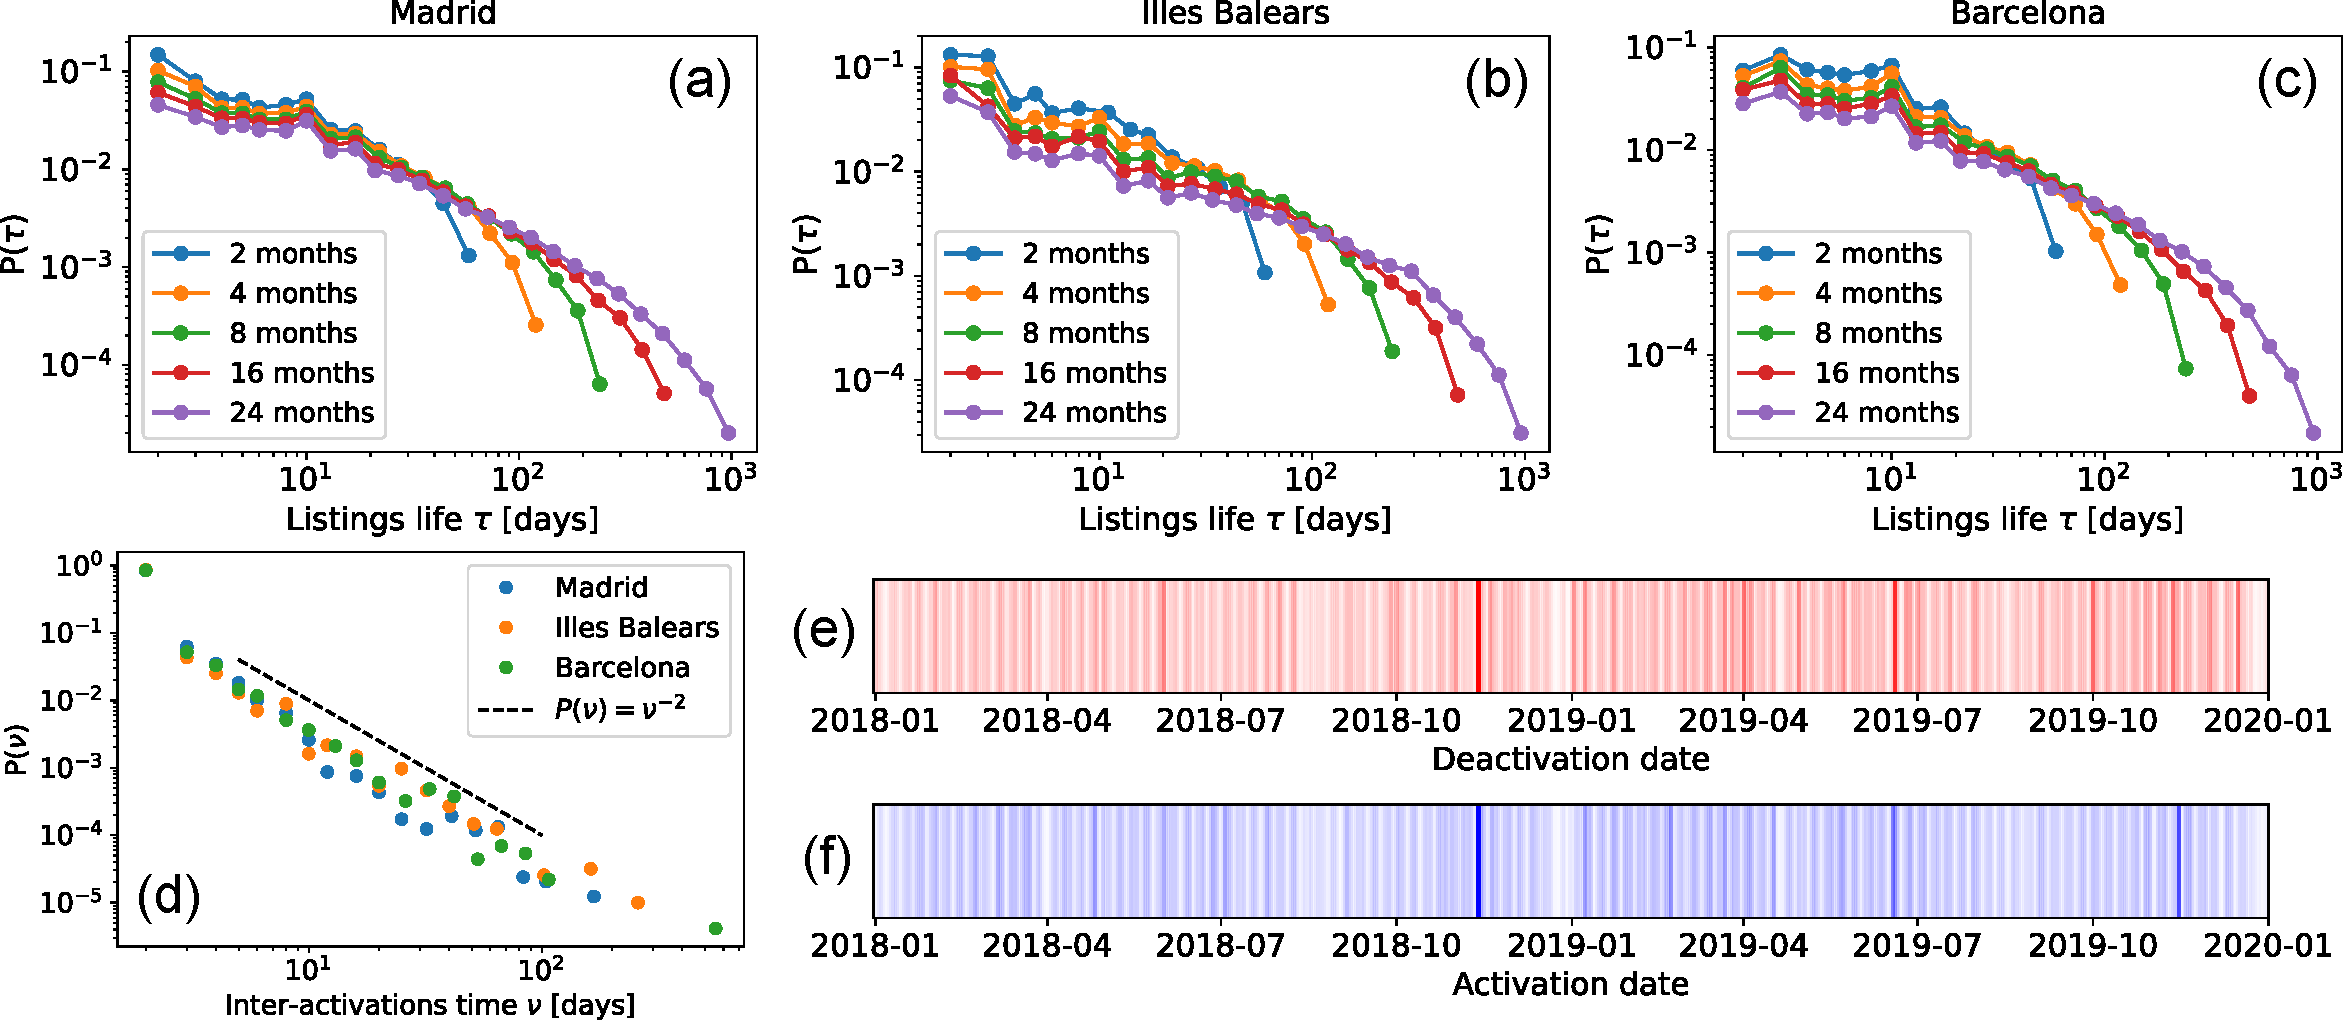
\includegraphics[width =\textwidth]{Figs/Idealista_dynamics/panel_time.pdf}
	\caption[Temporal statistics of the listing dynamics.]{ \label{fig:panel_time} Temporal statistics of the listing dynamics. Listings life (time posted in the platform) distribution for different time windows at Madrid \textbf{(a)}, Barcelona \textbf{(b)} and Balearic Islands \textbf{(c)}. Different colors indicate different time windows. \textbf{(d)} Inter-activations time distribution for the 3 regions. Different colors indicate different region or province. The dashed black line shows a $\nu^{-2}$ power-law distribution. \textbf{(e)} and \textbf{(f)} show the bar sequence of the adds deactivations and activations, respectively, for the Balearic Islands market. The color intensity indicates the number of adds.}
\end{figure}

The active listings dynamics is governed by the listings' life, defined as the number of days a certain listing has been posted in the platform. This measure is a proxy of a listings attractiveness, because when a listing is sold/rented, the agency removes it from the platform. This is an obvious simplification of the reality, since there are many scenarios: a listing removed because a personal decision of the owner, a listing available for long time because the demand is low, etc. However, in this analysis, we assume that when an agency removes a listing, it is because it has been sold/rented, which is the typical scenario. Fig. \ref{fig:panel_time}(a-c) shows the listings' life distribution for the 3 regions studied. The purple line is the distribution for a time window including the whole period (2 years). In all cases, the listings' life distribution shows a fat tail distribution, indicating that, even though there are a lot of listings that are sold in a few days, there are a few present for long periods of time. This heterogeneous life distribution is a signature of the burstiness of the listings' dynamics, what makes this system another example of the irregular human activity patterns mentioned in previous chapters of this thesis.

However, bursty dynamics are usually characterized by fat tail inter-event time distributions. For the listings' dynamics, when we explore the inter-activations time distributions (time between new listings activations) we find a power-law distribution with exponent $\gamma = -2$ for all regions, as shown in Fig. \ref{fig:panel_time}(d). When we compare this distribution with the inter-event time distribution of human activity patterns (with an exponent typically around $\gamma = -1$), we find that the listings' dynamics are less heterogeneous. A similar behavior is found in Fig. \ref{fig:panel_time}(e-f), where we show the bar sequence of the adds deactivations and activations for the Balearic Islands market. Even though we differentiate an irregular temporal dynamics on top of the weakly pattern, with days when there are more listings added or removed, the overall activation behavior is not as bursty as in other human activities. Therefore, the listings' dynamics show a high heterogeneous life distribution, but a less heterogeneous inter-event time distribution.

This process can be understood with the idea of ``aging'': Listings are added to the platform at some constant rate, highlighted by the linear increase of the total listings. But, the longer a listing is in the platform, the less likely it is to be sold/rented, motivated by the fat tail life distribution. In this particular scenario, aging does not reflect the attachment to a previous belief, as in the models in the previous part. Instead, aging acts as a time-changing attractiveness of the listing. This stochastic process is known in the literature as \textit{delayed degradation}, in which particles are added to a system at a constant rate, and they die after a certain time $\tau$ after being created. This time $\tau$ is usually allowed to be randomly distributed. This process has been studied in many situations, such as gene regulation \cite{}, neuronal activity \cite{}, and physiological processes \cite{}. In general, the delayed degradation stochastic process is solved in Ref. \cite{LaFuerza2013} but only for life distributions with a well-defined mean. In our case, the life distribution is fat-tailed, and the delayed degradation process needs to be treated with more detail.

\section{Agencies dynamics}

In previous section, we have analyzed the listings' dynamics, just exploring how the total and active adds increase in size. However, the listings are not isolated entities, but they have a price, a location and are posted by a real estate agency. In this section, we focus on the decision-making process that house owners follow when they decide to sell/rent their properties through a real estate agency, and how it is correlated with the pricing and the location of the listings.

\begin{figure}
    \vspace{0.2 cm}
    \centering
    \includegraphics[width = 0.8\textwidth]{Figs/Idealista_dynamics/temporal_bipartite.pdf}
	\caption[Housing market as a temporal bipartite network.]{Schematic representation of the temporal bipartite network between listings and agencies. On top, there is a temporal period in which the different listings are represented by colored horizontal lines, a representation of the time listings have been active in the platform. The color of the listings represent the real estate agency that posted them. For each time window, represented by purple and grey boxes (from $t_0$ to $t_f$), we build a bipartite network where listings are connected to the agency that posted it if the listing is active inside the temporal window. The colored big circles represent the agencies' nodes and the black small circles, the listings active posted. \label{fig:temporal_bipartite}}
\end{figure}

To this end, we build a temporal bipartite network between listings and agencies. At each time window, defined by an initial date $t_0$ and a final date $t_f$, we construct a bipartite network where listings are connected to the agency that posted it if the listing is active in any time $t'$, inside the temporal window $t_0 \leq t' \leq t_f$. Does not matter if the listing was removed after $t_f$ or if it was added before $t_0$, we consider active listings in the time window. Note that this network is very simple, as a listing cannot be connected to more than one agency. As it is observed in the schematic representation of the temporal bipartite network in Fig. \ref{fig:temporal_bipartite}, as the window moves in time, the bipartite network changes structure, allowing us to infer the dynamics listings-agencies.



\subsection{Preferential attachment}

\begin{figure}
    \label{fig:panel_degree}
    \centering
    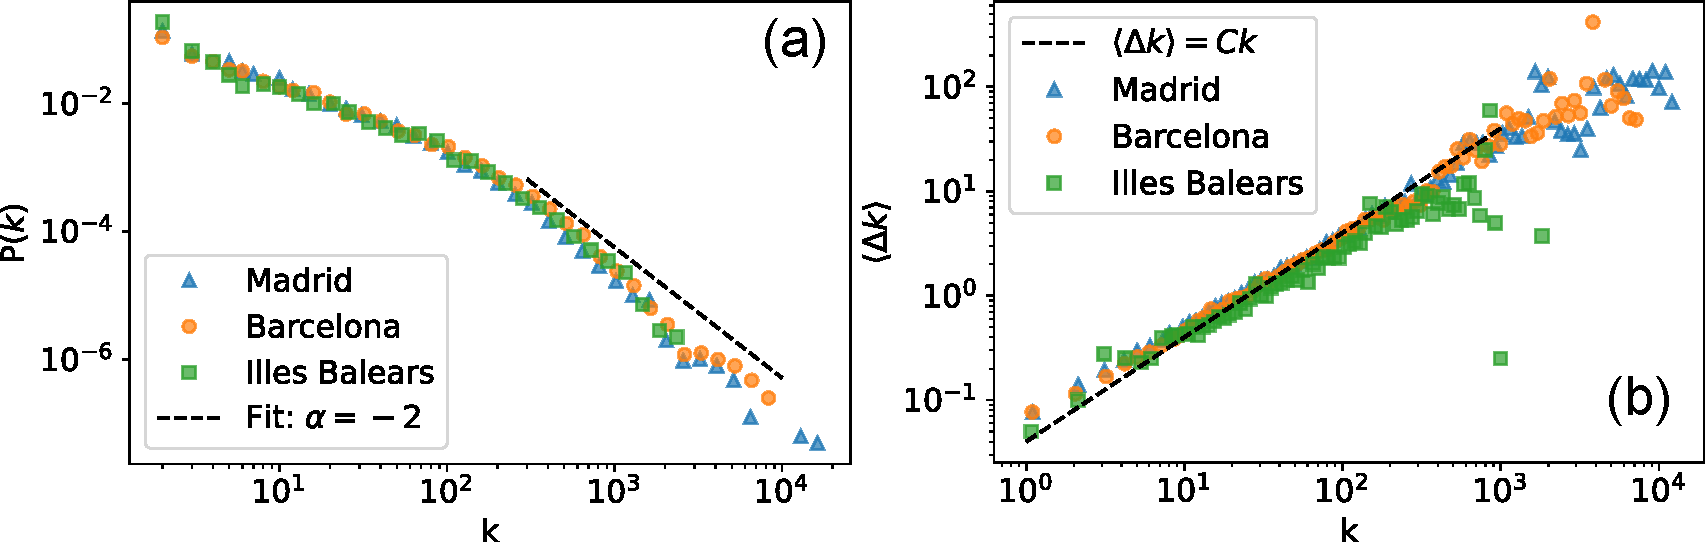
\includegraphics[width =\textwidth]{Figs/Idealista_dynamics/panel_degree.pdf}
	\caption[Preferential attachment to agencies.]{Preferential attachment to agencies. \textbf{(a)} Degree distribution of the agencies in the 3 regions. \textbf{(b)} Average degree increase of an agency as a function of the degree (listings posted) of the agency previously to the attachment. For both plots, different colors and markers indicate different regions or provinces. In \textbf{(a)}, the black dashed line shows a power-law distribution with exponent $\alpha  =-2$, and in \textbf{(b)} shows a linear increase with fitted slope $C = 0.04$.}
\end{figure}

\subsection{Price correlations}

\begin{figure}
    \label{fig:sigma_price}
    \centering
    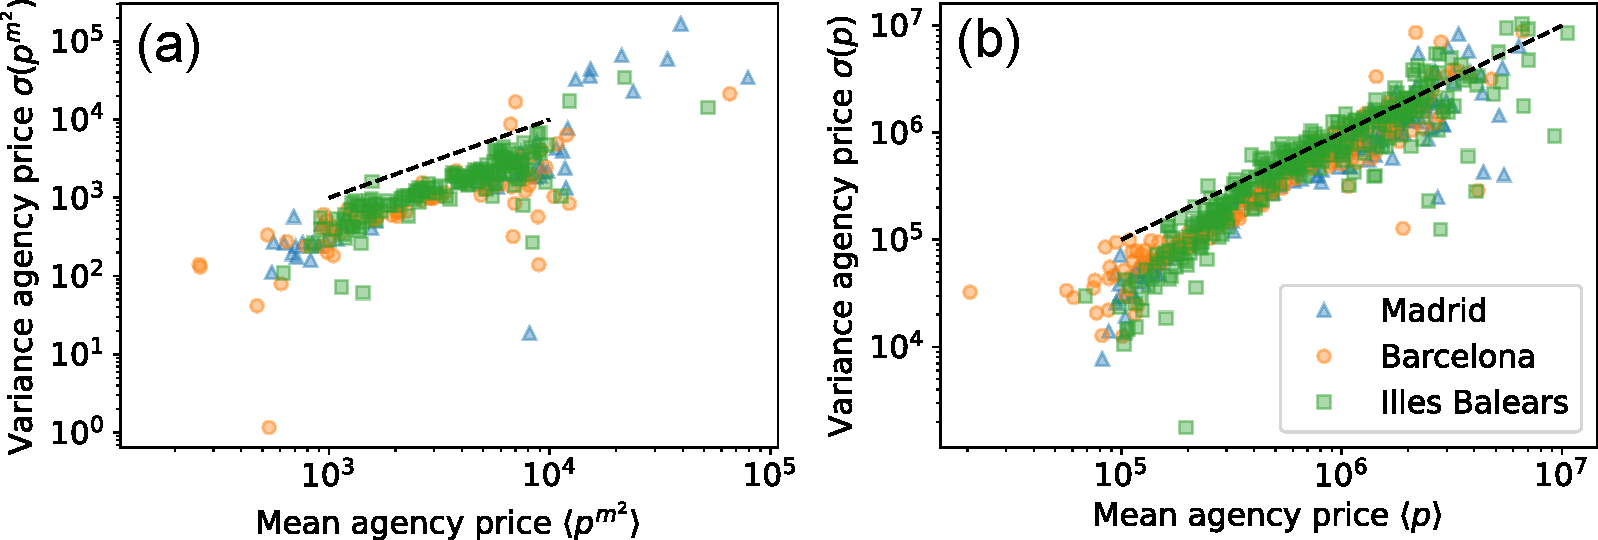
\includegraphics[width =\textwidth]{Figs/Idealista_dynamics/labeled_sigma_price.pdf}
	\caption[Variance of the agency price vs mean agency price.]{Variance of the listings price posted by an agency as a function of its mean price for the price per square meter \textbf{(a)} and the total price \textbf{(b)}. Different colors and markers indicate different regions or provinces. The black dashed line shows a linear fit with $\sigma = p^{{m}^2}$ for both plots.}
\end{figure}

\begin{figure}
    \label{fig:panel_price}
    \centering
    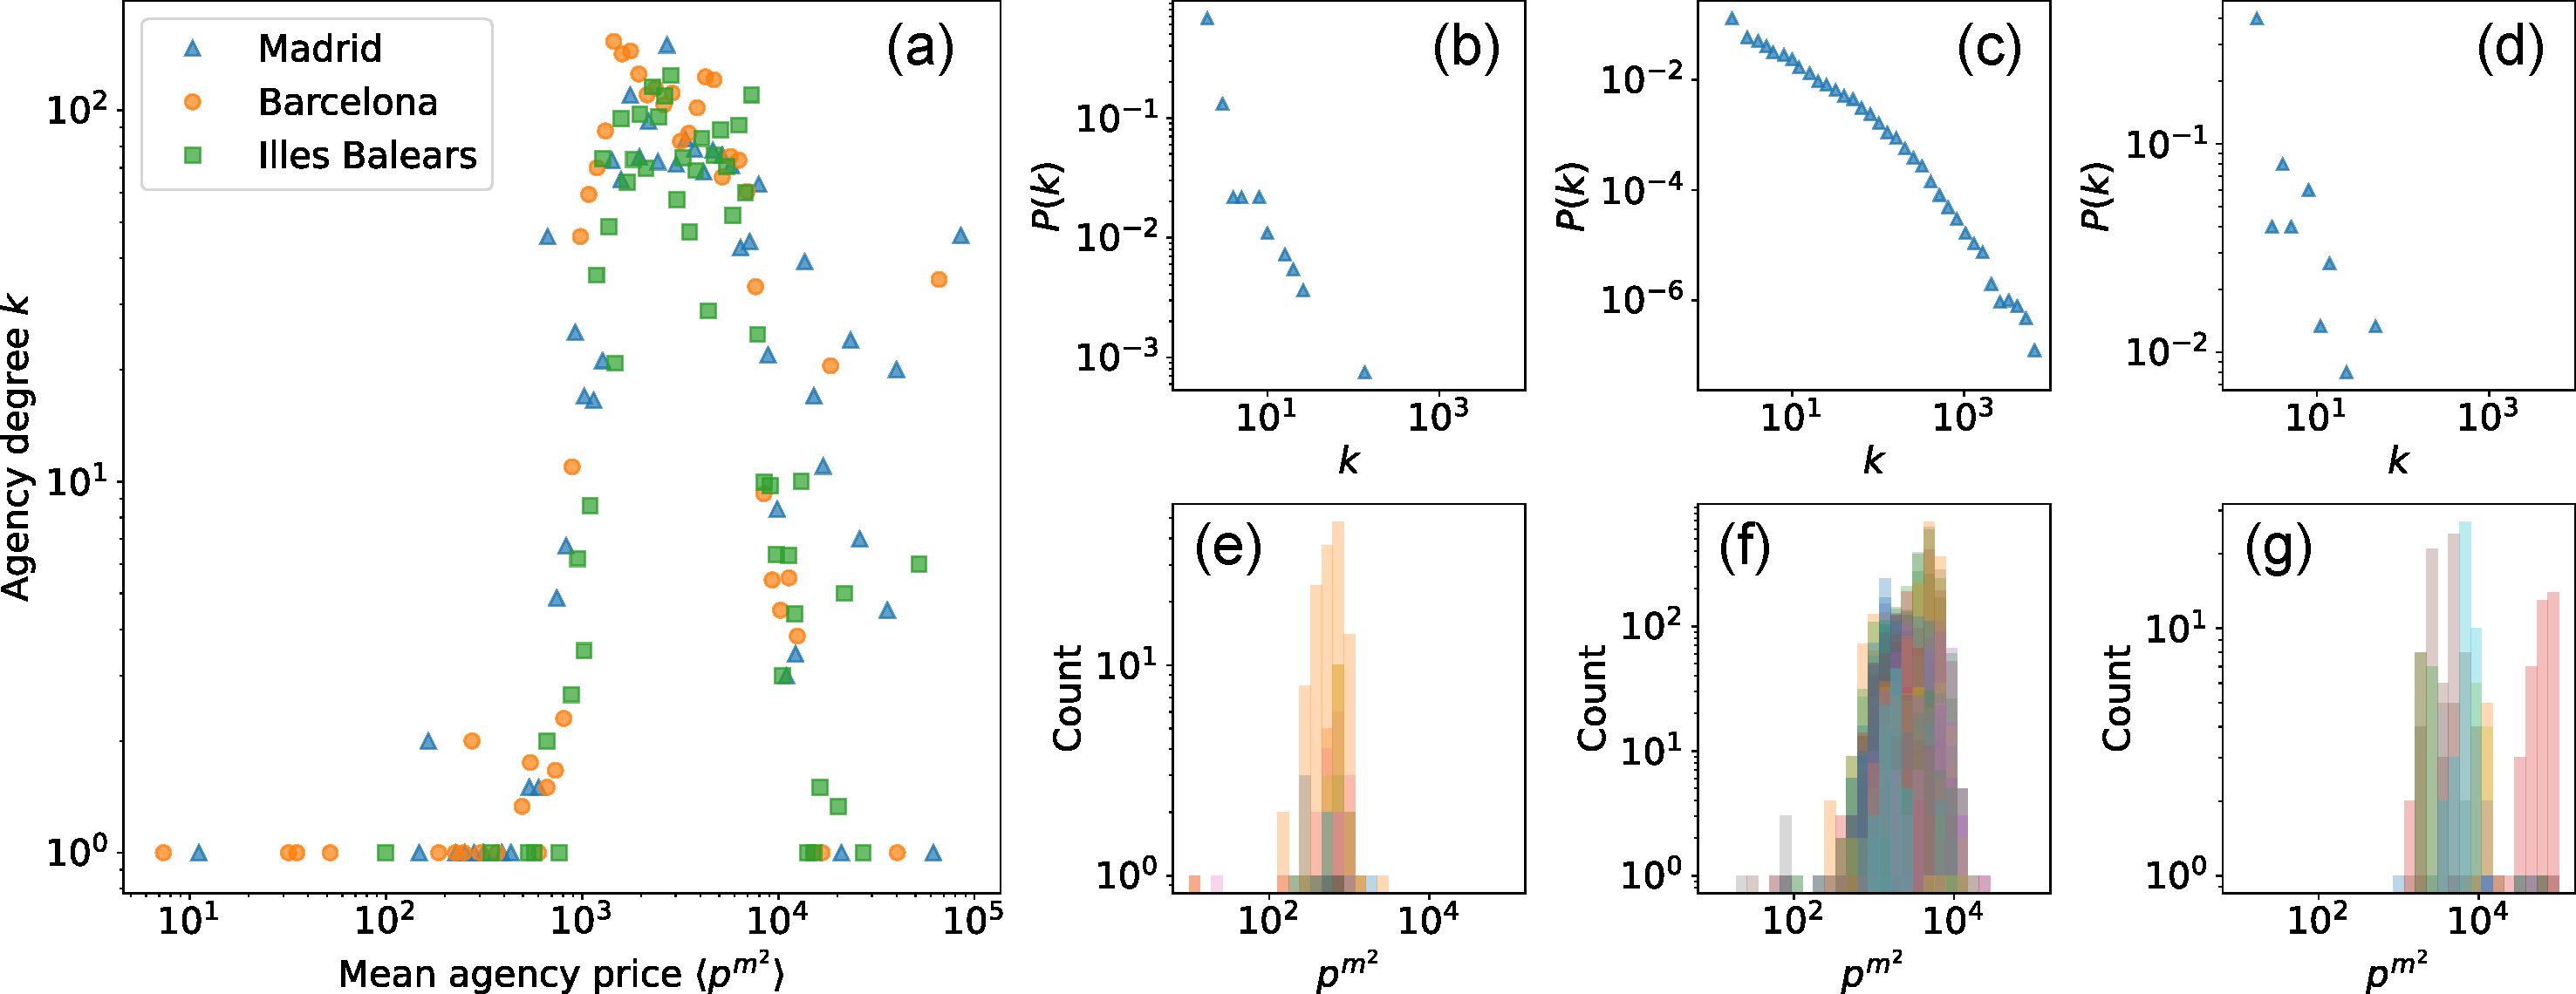
\includegraphics[width =\textwidth]{Figs/Idealista_dynamics/panel_price.pdf}
	\caption[Price segmentation by the degree.]{\textbf{(a)} Average degree (number of listings) of an agency as a function of its mean price per square meter. Different colors and markers indicate different regions or provinces. Degree distribution among the agencies \textbf{(b)-(c)-(d)} and price histograms for 60 representative agencies \textbf{(e)-(f)-(g)} at the different price segments: \textbf{(b)-(e)} $p^{{m}^2} < 800 \, \textup{\euro} / m^2$, \textbf{(c)-(f)} $800 \, \textup{\euro}  / m^2 < p^{{m}^2} < 10^4 \, \textup{\euro}  / m^2$, and \textbf{(d)-(g)} $p^{{m}^2} > 10^4 \, \textup{\euro}  / m^2$. These plots correspond to the Madrid housing market. For the price distributions, the colors indicate histograms for different agencies.}
\end{figure}

\begin{figure}
    \label{fig:attach_price}
    \centering
    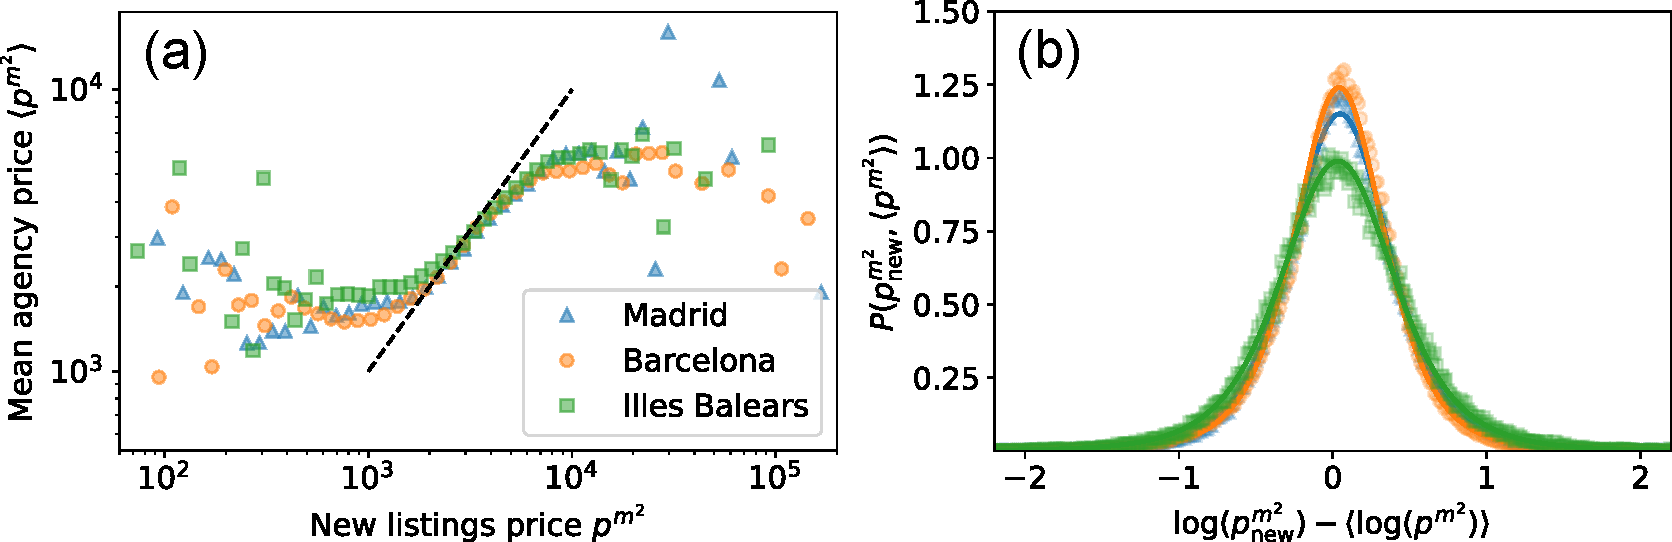
\includegraphics[width =\textwidth]{Figs/Idealista_dynamics/panel_attach_price.pdf}
	\caption[Attachment dynamics of new listings by price.]{Attachment of new listings by price. \textbf{(a)} Mean agency price per square meter as a function of the price of the new listing attached to the agency. Different colors and markers indicate different regions or provinces. The black dashed line shows a linear increase $\langle p^{{m}^2} \rangle = p^{{m}^2}$. \textbf{(b)} Distribution of the logarithmic difference between the price of the new listing and the mean price of the agency. Different colors indicate different regions or provinces. Each solid colored line corresponds to a T-student fit for each region. The parameters are: $\mu = 0.02$, $\sigma = 0.5$ for Madrid, $\mu = 0.02$, $\sigma = 0.5$ for Barcelona, and $\mu = 0.02$, $\sigma = 0.5$ for the Balearic Islands.}
\end{figure}

\subsection{Specialization}

\begin{figure}
    \label{fig:distance_panel}
    \centering
    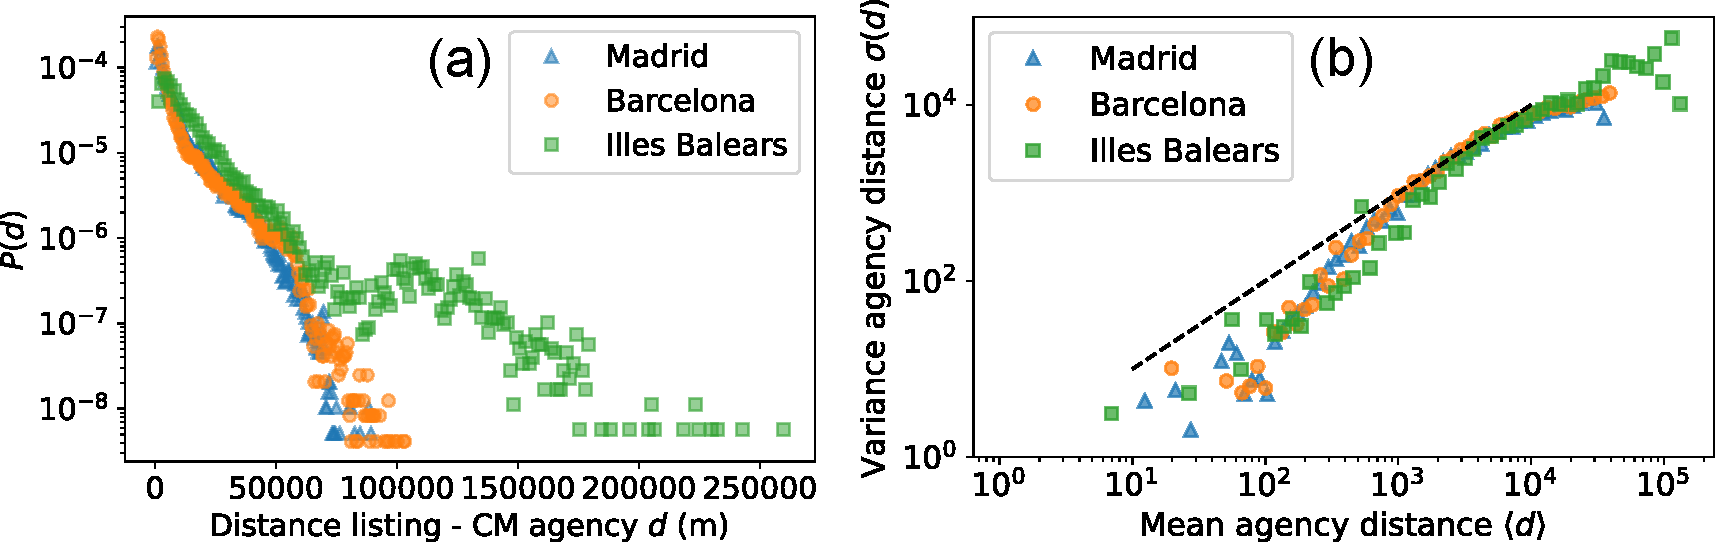
\includegraphics[width =\textwidth]{Figs/Idealista_dynamics/distance_panel.pdf}
	\caption[Distance correlations.]{\textbf{(a)} Distribution of the distance between listings of a certain agency and the agency center of mass (mean location of the listings posted by the agency). Different colors indicate different regions or provinces. \textbf{(b)} Variance of the listings distance to the agency center of mass of an agency as a function of the mean distance of that same agency. Different colors indicate different regions or provinces. The black dashed line shows a linear increase $\sigma(d) = \langle d \rangle$. }
\end{figure}

\begin{figure}
    \label{fig:distance_attach}
    \centering
    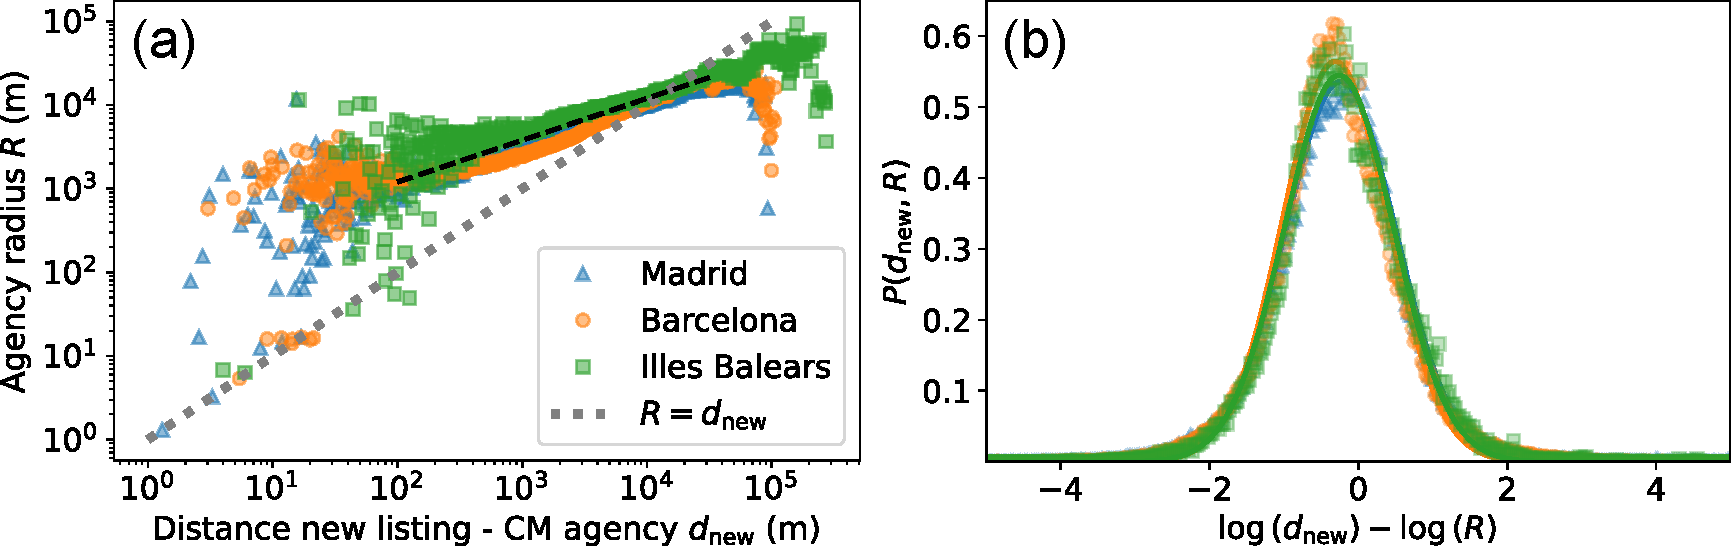
\includegraphics[width =\textwidth]{Figs/Idealista_dynamics/distance_attach.pdf}
	\caption[Attachment dynamics of new listings by distance.]{ Attachment dynamics of new listings by distance. \textbf{(a)} Agency radius (mean distance of the listings to the agency center of mass) as a function of the distance of the new listing (to the center of mass) attached to the agency. Different colors indicate different regions or provinces. The black dotted grey line shows a linear increase $R = d_{\rm new}$, while the dashed black line shows a square root dependence $R = C \, d_{\rm new}^{1/2}$ with $C = 120$. \textbf{(b)} Distribution of the logarithmic difference between the distance of the new listing and radius of the agency. Different colors indicate different regions or provinces. Each solid colored line corresponds to a T-student fit for each region. The parameters are: $\mu = 0.02$, $\sigma = 0.5$ for Madrid, $\mu = 0.02$, $\sigma = 0.5$ for Barcelona, and $\mu = 0.02$, $\sigma = 0.5$ for the Balearic Islands.}
\end{figure}

\section{Conclusions}












